\documentclass{amsbook}
\usepackage{../HBSuerDemir}

\begin{document}
    \hPage{b2p1/119}
    
    Line vectors can be expressed analytically by the use of coordinate systems. This representation will be called a \underline{coordinate vector}. Coordinate vectors are more convenient in all analytical treatments than the line vectors. We introduce below rectangular coordinate system to define coordinate vectors.\\
    
    \underline{Rectangular coordinate systems}:\\
    
    Consider in 3-space three mutually perpendicular axes $O_x$, $O_y$, $O_z$ with a common origin $O$, called a \underline{rectangular} (or \underline{cartesian}) \underline{coordinate system}, written $O_x_y_z$. A 3-space provided with such a system will be called an \underline{analytic 3-space}.\\
    
    In the following two figures two distinct coordinate systems are shown:\\
    
    \begin{minipage}[c]{0.5\textwidth}
            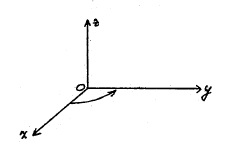
\includegraphics[width=0.6\textwidth]{images/b2p1-119-fig01.jpg}
            \begin{center}
                \raggedright\caption{A positive system\\ (A right hand system)}
            \end{center}
    \end{minipage}
    \hfill
    \begin{minipage}[c]{0.5\textwidth}
            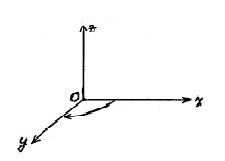
\includegraphics[width=0.6\textwidth]{images/b2p1-119-fig02.jpg}
            \begin{center}
                \raggedright\caption{A negative system \\ (A left hand system)}
            \end{center}
    \end{minipage}\\ \\
    
    On a positive system an observer, standing on $O_x_y$ plane at $O$ along positive z-axis observes that the angle from positive x-axis to positive y-axis is positive (counterclockwise). In a negative system the same observer observes that the same angle is negative (clockwise).\\
    
    The positiveness and negativeness is invariant under any translation and rotation of the coordinate axes.\\
    
    In this book we will always use positive systems.
    
\end{document}